\chapter{Causal Inference}

    \minitoc

\section{Causal DAGs}

    \newdef{Bayesian network}{\index{Bayesian!network}
        Consider a DAG $\mathcal{G}\equiv(V,A)$. A probability distribution $P$ is said to factorize over $\mathcal{G}$ if it can be written as:
        \begin{gather}
            P(V) = \prod_{x\in V}P\bigl(x\mid\mathrm{parents}(x)\bigr)\,.
        \end{gather}
    }

    \newdef{Mediator}{\index{mediator}
        Consider the DAG
        \begin{gather*}
            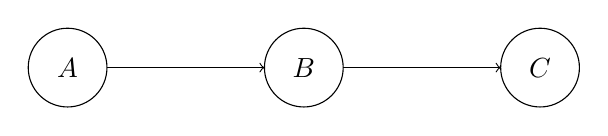
\begin{tikzpicture}
                \draw (0, 0) circle (0.5) node{$A$};
                \draw (3, 0) circle (0.5) node{$B$};
                \draw (6, 0) circle (0.5) node{$C$};
                \draw[->] (0.5, 0) -- (2.5, 0);
                \draw[->] (3.5, 0) -- (5.5, 0);
            \end{tikzpicture}
        \end{gather*}
        The variable $B$ is called a mediator for $A$ and $C$.
    }
    \newdef{Fork}{\index{fork}
        A DAG of the form
        \begin{gather*}
            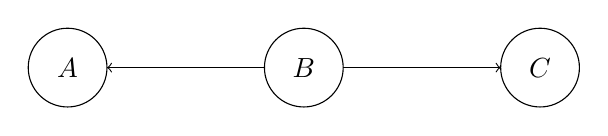
\begin{tikzpicture}
                \draw (0, 0) circle (0.5) node{$A$};
                \draw (3, 0) circle (0.5) node{$B$};
                \draw (6, 0) circle (0.5) node{$C$};
                \draw[<-] (0.5, 0) -- (2.5, 0);
                \draw[->] (3.5, 0) -- (5.5, 0);
            \end{tikzpicture}
        \end{gather*}
    }
    \newdef{Collider}{\index{collider}
    A DAG of the form
        \begin{gather*}
            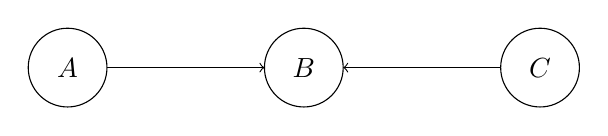
\begin{tikzpicture}
                \draw (0, 0) circle (0.5) node{$A$};
                \draw (3, 0) circle (0.5) node{$B$};
                \draw (6, 0) circle (0.5) node{$C$};
                \draw[->] (0.5, 0) -- (2.5, 0);
                \draw[<-] (3.5, 0) -- (5.5, 0);
            \end{tikzpicture}
        \end{gather*}
    }

    \newdef{$d$-separation}{\index{separation}\index{blocked}
        Consider a DAG $\mathcal{G}\equiv(V,A)$. Two subsets $V_1,V_2\subset V$ are said to be $d$-separated by a set $V_3\subset V$ whenever all paths from $V_1$ to $V_2$ are blocked by $V_3$. A path is said to be \textbf{blocked} whenever at least one mediator or fork ancestor on the path is contained in $V_3$ or at least one of the colliders on the path is not contained in $V_3$. 
    }
    \begin{property}
        Consider a Bayesian network represented by the DAG $\mathcal{G}\equiv(V,A)$. If $V_1,V_2\subset V$ are $d$-separated by $V_3\subset V$, then $V_1\indep V_2\mid V_3$.
    \end{property}

    \newdef{Causal path}{\index{causal!path}
        A path in a DAG such that all arrows point in the same direction.
    }

    Combining the notions of $d$-separation and causality leads to formulas that allow to separate `spurious' correlations from actual causal relations. Consider for example the collider diagram. As long as the value of $B$ is not fixed, the variables $A$ and $C$ are independent. However, in each stratum of $B$, the values of $A$ and $C$ might be correlated, although they are not causally related.

\section{Do-calculus}\index{do-calculus}

    In this section, $\mathbf{G}$ will always denote a DAG characterizing the underlying causal model.

    \begin{axiom}[Insertion and deletion of variables]
        If $X,Z$ are $d$-separated by $X,W$ in $\mathbf{G}_X$, the subgraph obtained from $\mathbf{G}$ by removing all arrows pointing to $X$, then
        \begin{gather}
            P\bigl(Y\mid\mathrm{do}(X),Z,W\bigr) = P\bigl(Y\mid\mathrm{do}(X),W\bigr)\,.
        \end{gather}
    \end{axiom}

    \begin{axiom}[Exchange of action and observation]
        If $Y,Z$ are $d$-separated by $X,W$ in $\mathbf{G}_X^Z$, the subgraph obtained from $\mathbf{G}$ by removing all arrows pointing to $X$ and all arrows pointing from $Z$, then
        \begin{gather}
            P\bigl(Y\mid\mathrm{do}(X),\mathrm{do}(Z),W\bigr) = P\bigl(Y\mid\mathrm{do}(X),Z,W\bigr)\,.
        \end{gather}
    \end{axiom}

    \begin{axiom}[Insertion and deletion of actions]
        If $X,Z$ are $d$-separated by $X,W$ in $\mathbf{G}^*$, the subgraph obtained from $\mathbf{G}$ by removing all arrows pointing to $X$ and all arrows pointing to $Z$ that are not ancestors of $W$ in $\mathbf{G}_X$, then
        \begin{gather}
            P\bigl(Y\mid\mathrm{do}(X),\mathrm{do}(Z),W\bigr) = P\bigl(Y\mid\mathrm{do}(X),W\bigr)\,.
        \end{gather}
    \end{axiom}

    \todo{COMPLETE}